\documentclass{beamer}

\usepackage{tikz}
\usepackage{amsmath}
\usepackage{amssymb}
\usepackage{amsfonts}
\usepackage{amsthm}
\usepackage{tikz}
\usepackage{float}
\usepackage[T1]{fontenc}

\addtobeamertemplate{navigation symbols}{}{%
    \usebeamerfont{footline}%
    \usebeamercolor[fg]{footline}%
    \hspace{1em}%
    \raisebox{1.5pt}[0pt][0pt]{\insertframenumber/\inserttotalframenumber}
}

\usetikzlibrary{positioning}
\usetikzlibrary{arrows.meta}

\setbeamertemplate{bibliography item}{}

\bibliographystyle{abbrv}

\title{An Introduction to Chaos in Topological Dynamical Systems}
\author{Fraser Robert Love}
\institute{School of Mathematics and Statistics \\ University of St Andrews}
\date{March 27, 2023}

\begin{document}

\frame{\titlepage}

\begin{frame}
    \frametitle{Table of Contents}
    \tableofcontents
\end{frame}

\section{Topological Dynamics}
\begin{frame}
    \frametitle{Topological Dynamics}

    \begin{block}{Definition (Topological Dynamical System).}
        \begin{itemize}
            \item Let $X$ be a non-empty compact metric space. A \emph{topological dynamical system}, denoted $(X, f)$, is given by a continuous map $f: X \to X$. 
            \item The system starts at an initial point $x \in X$ and evolves through successive iterations of the map $f$.
            \item After $k \in \mathbb{N}$ iterations of $f$, the system can be described by $f^n := f \circ f \circ \dots \circ f$, where $x$ is mapped to the point $f^n(x)$.
        \end{itemize}
    \end{block}
\end{frame}

\begin{frame}
    \frametitle{Topological Dynamics}

    \begin{block}{Definition (Orbit).}
        Let $(X, f)$ be a topological dynamical system. The \emph{orbit} of $x \in X$ under $f$ is the set $\mathcal{O}_f(x) = \lbrace f^n(x) : n \geq 0 \rbrace = \lbrace x, f(x), f^2(x), \dots \rbrace$ of iterates of $x$ under the map $f$.
    \end{block}

    \begin{block}{Definition (Periodic Point, Cycle).}
        \begin{itemize}
            \item Let $(X, f)$ be a topological dynamical system. A point $x \in X$ is \emph{periodic} if $f^n(x) = x$ for some $n \in \mathbb{N}$.
            \item The \emph{period} of a point $x$ is the least positive integer $k$ such that $f^k(x) = x$. If $x$ has a period of $k$ we say that $x$ is a \emph{period-$k$} point.
            \item The orbit $\mathcal{O}_f(x) = \lbrace x, f(x), \dots, f^{k-1}(x) \rbrace$ of a periodic point is a finite set of unique points, called a \emph{periodic orbit} of period $k$ or simply a \emph{k-cycle}.
        \end{itemize}
    \end{block}
\end{frame}

\begin{frame}
    \frametitle{Topological Dynamics}

    \begin{block}{Example (Logistic Map).}
        Define $F_{\mu}: [0, 1] \to [0, 1]$ to be the \emph{logistic map}, where $F_{\mu}(x)=\mu x(1-x)$ and $\mu > 0$.
        
        \begin{figure}[h]
            \centering
            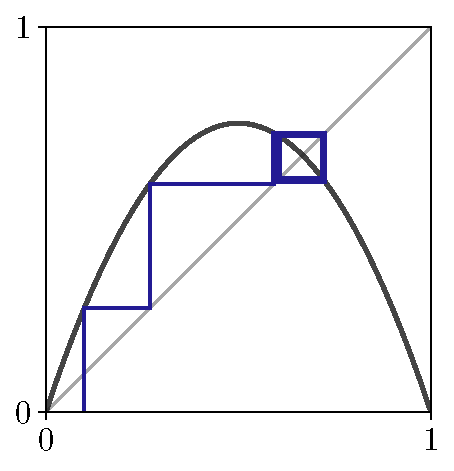
\includegraphics[width=4.5cm]{../images/logistic_3_0.1}
            \caption{Logistic map $F_\mu$ with $\mu = 3$.}
            \label{fig:logistic_3}
        \end{figure}

    \end{block}
\end{frame}

\begin{frame}
    \frametitle{Topological Dynamics}

    \begin{block}{Example (Doubling Map).}
        Define $\mathcal{D}: S^1 \to S^1$ to be the \emph{doubling map on} $S^1 = \left\lbrace z \in \mathbb{C}: |z| = 1 \right\rbrace$, where $\mathcal{D}(z) = z^2$, or equivalently $\mathcal{D}(e^{i\theta}) = e^{2i\theta}$ for some $\theta \in \mathbb{R}$.

        \begin{figure}[h]
            \centering
            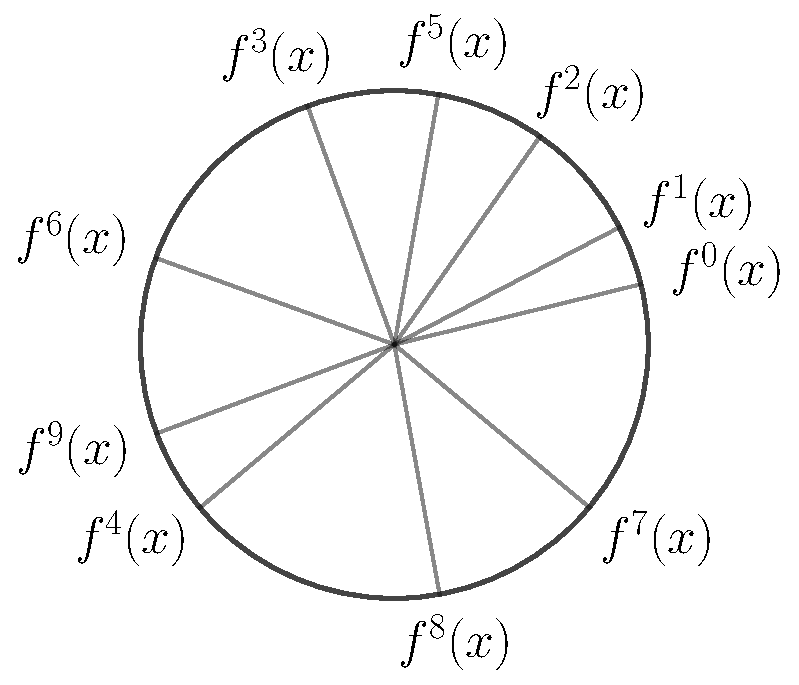
\includegraphics[width=5cm]{../images/doubling_circle}
            \caption{First ten iterations of the doubling map $\mathcal{D}$.}
            \label{fig:doubling-circle}
        \end{figure}
    \end{block}
\end{frame}

\begin{frame}
    \frametitle{Topological Dynamics}
    \begin{block}{Definition (Sequence Space).}
        \begin{itemize}
            \item Let $\Sigma_2 = \left\lbrace (s_1, s_2, \dots): s_i \in \left\lbrace 0, 1 \right\rbrace \right\rbrace$ be the set sequences of ones and zeros.
            \item Define $(\Sigma_2, d)$ to be the \emph{sequence space} where $d(s, t) = \Sigma_{i=1}^{\infty}|s_i - t_i|2^{-i}$ is a metric for $(s)_{i=1}^{\infty}, \ (t)_{i=1}^{\infty}  \in \Sigma_2$.
            \item The sequence space $(\Sigma_2, d)$ is compact.
        \end{itemize}
    \end{block}
\end{frame}

\begin{frame}
    \frametitle{Topological Dynamics}
    \begin{block}{Proposition.}
        The \emph{shift map} $\sigma: \Sigma_2 \to \Sigma_2$ given by $\sigma \left((s)_{i=1}^{\infty}\right) = (s)_{i=2}^{\infty}$ is continuous.
        \begin{proof}
            Let $\varepsilon > 0$ and choose $\underline{s} = (s_i)_{i=1}^{\infty}, \ \underline{t} = (t_i)_{i=1}^{\infty} \in \Sigma_2$ such that $d(\underline{s}, \underline{t}) = \Sigma_{i=1}^{\infty}|s_i - t_i|2^{-i} < \delta$. Choose $n$ such that $2^{-n} \leq \varepsilon$ and let $\delta = 2^{-(n+1)}$. Hence $\underline{s}$ and $\underline{t}$ agree on the first $n+1$ symbols and $\sigma\left(\underline{s}\right)$ and $\sigma\left(\underline{t}\right)$ agree on the first $n$ symbols. Then $d\left( \sigma\left(\underline{s}\right), \sigma\left(\underline{t}\right) \right) = d\left((s)_{i=n+1}^{\infty}, (t)_{i=n+1}^{\infty}\right) = \Sigma_{i=n+1}^{\infty}|s_i - t_i|2^{-i} \leq 2^{-n} \leq \varepsilon$.
        \end{proof}
    \end{block}
    \vspace{0.5cm}
    Hence $(\Sigma_2, \sigma)$ defines a topological dynamical system.
\end{frame}

\section{Introduction to Chaos}

\begin{frame}
    \frametitle{Introduction to Chaos}
    \begin{itemize}
        \item Many different definitions of chaos exist for topological dynamical systems.
        \item Devaney chaos, Li-Yorke chaos, Topological chaos, etc.
        \item These definitions rely on many different topological characteristics to define chaos in a natural way.
        \item We will focus on Devaney chaos and the characteristics of topological transitivity / existence of a dense orbit, sensitive dependence on initial conditions and dense periodic points.
    \end{itemize}
\end{frame}

\section{Topological Characteristics of Chaos}
\begin{frame}
    \frametitle{Topological Characteristics of Chaos}
    \begin{block}{Definition (Topological Transitivity).}
        Let $(X, f)$ be a topological dynamical system. The map $f$ is \emph{topologically transitive} if for every pair of non-empty open sets $U, V \subseteq X$ there exists $k > 0$ such that $f^k(U) \cap V \neq \emptyset$.
    \end{block}
    \vspace{0.3cm}
    In a topologically transitive mapping, points in an arbitrarily small set can be mapped into any other arbitrary small set under a repeated number of iterations of the map.
    \vspace{0.3cm}
    \begin{block}{Proposition.}
        Let $(X, f)$ be a topological dynamical system and suppose $X$ has no isolated points. The map $f$ is topologically transitive if and only if there exists some $x \in X$ such that $\mathcal{O}(x)$ is dense in $X$. \cite{silverman}
    \end{block}
\end{frame}

\begin{frame}
    \frametitle{Topological Characteristics of Chaos}
    \begin{block}{Proposition.}
        The shift map $(\Sigma_2, \sigma)$ is topologically transitive. \cite{devaney}
        \begin{proof}
            Let $\underline{t} = (t)_{i=0}^{\infty} \in \Sigma_2$ be arbitrary and $\varepsilon > 0$. Consider the sequence $\underline{s} = (0, 1, \{0, 0\}, \{0, 1\}, \{1, 0\}, \{1, 1\}, \{0, 0, 0\}, \{0, 0, 1\}, \dots)$ of 0s and 1s sorted in len-lex order. By construction we can perform some $k \in \mathbb{N}$ iterations of $\sigma$ such that the first $n$ symbols of $\sigma^k(\underline{s})$ and $\underline{t}$ agree. Choose $N \geq \log_2{\frac{1}{\varepsilon}}$. Therefore for $n \geq N - 1$ we have that, $d(\sigma^k(\underline{s}), \underline{t}) = \sum_{i = n}^{\infty}|\sigma^k(\underline{s})_i - t_i|2^{-i} \leq 2^{-(n+1)} < 2^{-N} \leq \varepsilon$. Hence $\mathcal{O}(\underline{s})$ is dense in $\Sigma_2$ and so $(\Sigma_2, \sigma)$ is topologically transitive.
        \end{proof}
    \end{block}
\end{frame}

\begin{frame}
    \frametitle{Topological Characteristics of Chaos}
    \begin{block}{Definition (Sensitive Dependence on Initial Conditions).}
        Let $(X, f)$ be a topological dynamical system and $\varepsilon > 0$. A point $x \in X$ is \emph{$\varepsilon$-unstable} if, for every neighbourhood $U$ of $x$, there exists a point $y \in U$ and $k \geq 0$ such that $d\left(f^k(x), f^k(y)\right) \geq \varepsilon$. The map $f$ has \emph{sensitive dependence on initial conditions} if for all points $x \in X$, $x$ is $\varepsilon$-unstable.
    \end{block}
    \vspace{0.5cm}
    In other words, there exist points arbitrary close to $x$ that eventually get mapped at least $\varepsilon$ far apart under multiple applications of the map.
\end{frame}

\begin{frame}
    \frametitle{Topological Characteristics of Chaos}
    \begin{block}{Example.}
        The shift map $(\Sigma_2, \sigma)$ has sensitive dependence on initial conditions.
        \begin{proof}
            Take $\delta = 1$. Let $\underline{s} = (s)_{i=1}^{\infty} \in \Sigma_2$ and let $\varepsilon > 0$. Choose $n$ such that $2^{-n} < \varepsilon$. Pick $\underline{t} = (t)_{i=1}^{\infty} \in \Sigma_2$ such that $d(\underline{s}, \underline{t}) \leq 2^{-n} \leq \varepsilon$. Hence $\underline{s}$ and $\underline{t}$ agree on the first $n+1$ symbols. Now there exists a $k > n + 1$ such that $s_k \neq t_k$. The first term of $\sigma^k(\underline{s})$ is $s_k$ and the first term of $\sigma^k(\underline{t})$ is $t_k$. Therefore $d(\sigma^k(\underline{s}), \sigma^k(\underline{t})) = \sum_{i = 0}^{\infty}|s_{i+k} - t_{i+k}|2^{-i} \geq |s_k - t_k|2^{0} = 1 = \delta$.
        \end{proof}
    \end{block}
\end{frame}

\begin{frame}
    \frametitle{Topological Characteristics of Chaos}
    \begin{block}{Proposition.}
        The periodic points of the shift map $(\Sigma_2, \sigma)$ are dense in $\Sigma_2$. \cite{devaney}
    \begin{proof}
        Let $\underline{s} = (s)_{i=1}^{\infty}$ be an arbitrary point in $\Sigma_2$ and let $\varepsilon > 0$. Pick an $n$ such that $2^{-n} \leq \varepsilon$ and define $t_n = (s_0, \dots, s_n, s_0, \dots, s_n, \dots)$ to be an infinite repeating sequence where $t_i = s_i$ for $1 \leq i \leq n$. Then $d(s, t) = \sum_{i = 0}^n|s_i - t_i|2^{-i} + \sum_{i=n+1}^{\infty}|s_i - t_i|2^{-i} = \sum_{i = n+1}^{\infty}2^{-i} \leq 2^{-n} \leq \varepsilon$. Hence as $n \to \infty$ we have $t_n \to \underline{s}$. Since $\underline{s}$ was arbitrary, the periodic points of $\sigma$ are dense.
    \end{proof}
    \end{block}
\end{frame}

\section{Devaney Chaos}
\begin{frame}
    \frametitle{Devaney Chaos}
    \begin{block}{Definition (Devaney Chaos).}
        A topological dynamical system $(X, f)$ is \emph{chaotic in the sense of Devaney} if it is topologically transitive, has sensitive dependence on initial conditions, and if the periodic points of $f$ are dense in $X$.
    \end{block}
    \vspace{0.5cm}
    Devaney's definition considers:
    \begin{itemize}
        \item Unpredictability (sensitive dependence on initial conditions).
        \item Repetitiveness (dense periodic points).
        \item Indecomposability (topological transitivity).
    \end{itemize}
\end{frame}

\begin{frame}
    \frametitle{Devaney Chaos}
    \begin{block}{Proposition.}
        The shift map $(\Sigma_2, \sigma)$ is chaotic in the sense of Devaney.
        \begin{proof}
            We previously showed that $(\Sigma_2, \sigma)$ is topologically transitive (has a dense orbit), has sensitive dependence on initial conditions and has dense periodic points in $\Sigma_2$. Hence $(\Sigma_2, \sigma)$ is Devaney chaotic.
        \end{proof}
    \end{block}
\end{frame}

\section{Concluding Remarks}
\begin{frame}
    \frametitle{Concluding Remarks}
    \begin{itemize}
        \item We have defined chaos to be a mixture of unpredictability, repetitiveness and indecomposability.
        \item This was achieved using the properties of topological transitivity, sensitive dependence on initial conditions and dense periodic points.
        \item We have shown that the shift map $(\Sigma_2, \sigma)$ is a Devaney chaotic topological dynamical system.
        \item Using topological conjugacy we can use the fact that $(\Sigma_2, \sigma)$ is Devaney chaotic to prove that  $([0, 1], F_\mu)$, $(S^1, \mathcal{D})$ and many more systems exhibit Devaney chaos.
    \end{itemize}
\end{frame}

\section{Bibliography}
\begin{frame}
    \frametitle{Bibliography}
    \bibliography{../chaos}
\end{frame}

\end{document}